\documentclass[tikz]{standalone}

\usepackage[british]{babel}
\usepackage[utf8]{inputenc}
\usepackage{graphicx}
\usepackage{amsmath}
\usepackage{amssymb}
\usepackage{amsfonts}
\usepackage{bm}
\usepackage{color}
\usepackage[unicode]{hyperref}
\usepackage{multirow}
\usepackage{multicol}
\usepackage{tikz}
\usepackage{hyperref} % this is for url links
\usepackage{textcomp}
\usepackage{pgfplots}
\usetikzlibrary{calc,external,arrows,math}

%\usetikzlibrary{arrows,shapes}

\usepgfplotslibrary{polar}


\begin{document}
	%\begin{tikzpicture}
	%    \draw (-3,0) -- (3,0);
	%    \draw (-1.8,0) arc (160:90:4);
	%    \draw[dashed,very thick,red] (-1.8,0) arc (160:90:4);
	%    \draw[dashed,very thick,red] (-3,0) -- (-1.8,0);
	%    \draw[dashed,very thick,green] (-1.8,0) -- (3,0);
	%    
	%    \draw[gray] (-0.7,-0.8) node {substrate};
	%    \draw[gray] (0.5,-0.6) -- ++(-135:0.5) -- ++(0.3,0) arc (0:45:0.3) node[right] {$\alpha_1$};
	%    \draw[gray] (0.8,1.2) node {particle};
	%    \draw[gray] (2,1.4) -- ++(-115:0.5) -- ++(0.3,0) arc (0:65:0.3) node[right] {$\alpha_2$};
	%    \draw[gray] (-2.5,2) node {parent};
	%    
	%    \draw (-1.8,0) -- +(70:2);
	%    \draw (-1.8+0.4,0) arc (0:70:0.4);
	%    \draw[red] (-1.2,0.3) node {$\vartheta_2$};
	%    \draw[red] (-0.7,2.3) node {$\sigma_2(\vartheta_2)$};
	%    \draw[red] (-2.7,0.3) node {$\vartheta_1 = 180$\textdegree};
	%    \draw[red] (-2.7,-0.3) node {$\sigma_1(\vartheta_1)$};
	%    \draw (-1.8+0.3,0) arc (0:180:0.3);
	%    
	%    \draw[green] (0.8,0.3) node {$\vartheta_3=0$\textdegree};
	%    \draw[green] (0.8,-0.3) node {$\sigma_3=\mathrm{const}$};
	%\end{tikzpicture}
	%
	%\begin{tikzpicture}[scale=1,font=\normalsize]
	%    \def\figxwidth{3.5}
	%    \begin{axis}[
		%            axis equal,
		%            disabledatascaling,
		%            axis line style={draw=none},
		%            xtick=\empty,
		%            ytick=\empty,
		%            xmin=-\figxwidth,xmax=\figxwidth,
		%            declare function={
			%                % yshift1=0;
			%                yshift1=-0.6;
			%                n=4;
			%                nsoa=0.9;
			%                rot1 = 30;
			%                RW = 0.7*3;
			%                d=nsoa/(n^2-1);
			%                aniso1(\t)=1+d*cos(n*(\t-rot1));
			%                daniso1(\t)=-n*d*sin(n*(\t-rot1));
			%                Wulffx1(\t) = RW*( aniso1(\t)*cos(\t) - daniso1(\t)*sin(\t) );
			%                Wulffy1(\t) = RW*( aniso1(\t)*sin(\t) + daniso1(\t)*cos(\t) );
			%                },
		%        ]
		%        \begin{scope}
			%            \clip (axis cs: -\figxwidth,5) rectangle (axis cs:\figxwidth,0);
			%            \addplot[domain=-pi:pi, samples=150, smooth, thick] ({Wulffx1(deg(x))},{Wulffy1(deg(x))+yshift1});
			%            \addplot[domain=-pi:pi, samples=150, smooth, red, dash dot, thick] ({1.03*Wulffx1(deg(x))},{1.03*Wulffy1(deg(x))+yshift1});
			%        \end{scope}
		%        
		%        \begin{scope}
			%            \clip (axis cs: -\figxwidth,-5) rectangle (axis cs:\figxwidth,0);
			%            \addplot[domain=-pi:pi, samples=150, smooth,dashed] ({Wulffx1(deg(x))},{Wulffy1(deg(x))+yshift1});
			%        \end{scope}
		%        
		%        \path coordinate (C1) at (axis cs:0,yshift1);
		%        \path coordinate (B1) at (axis cs:-\figxwidth,0);
		%        \path coordinate (B2) at (axis cs:\figxwidth,0);
		%        \path coordinate (zz) at  (axis cs:0,0);
		%        
		%        % interfaxce specifications
		%        \draw (B1) -- (B2);
		%        \draw[red, dash dot, thick] (axis cs:-\figxwidth,0.05) -- node[midway, above] {$\sigma_{1}^L(\frac{\pi}{2})$} (axis cs:-1.9,0.05);
		%        \draw[red] (axis cs:0,1.4) node[above right] {$\sigma_{2}(\theta_{2})$} ;
		%        \draw[red, dash dot, thick] (axis cs:\figxwidth,0.05) -- node[midway, above] {$\sigma_{1}^R(-\frac{\pi}{2})$} (axis cs:2.1,0.05);
		%        \draw[blue, densely dotted, thick] (axis cs:-1.83,0.05) -- node [midway, above] {$\sigma_{3}=const$} (axis cs:2.0,0.05);
		%        
		%        \draw[stealth-stealth] (axis cs:-0.4,0) -- (axis cs:-0.4,yshift1/2) node [right] {$X_0 \Gamma$} -- (axis cs:-0.4,yshift1);
		%        
		%        \draw[fill] (C1) circle (1.5pt);
		%        
		%        % \draw (axis cs:-2.5,1.5) node [circle,draw,minimum size=6] {$\mathit{3}$};
		%        % \draw (axis cs:-1,0.8) node [circle,draw,minimum size=6] {$\mathit{2}$};
		%        % \draw (axis cs:-2.5,-1.5) node [circle,draw,minimum size=6]  {$\mathit{1}$};
		%        
		%        % \draw (axis cs: 0,0.8) -- ++(\rtheta{0.5cm}{-150}) -- ++(\rtheta{0.3cm}{0}) node [above right] {l} ;
		%        \draw (0.3,1.2) -- ++(-150:0.7) -- ++(0:0.3) node [right] {$\alpha_2$} arc (0:30:0.3) ;
		%        \draw (0.1,-1.1) -- ++(65-180:0.7) -- ++(0:0.3) node [right] {$\alpha_1$} arc (0:65:0.3) ;
		%    \end{axis}
	%\end{tikzpicture}
	%
	%

	%
	%\begin{tikzpicture}
	%    \draw[fill=blue!10] (0,0) rectangle (3,3);
	%    \foreach \i/\j in {0/1,1/2,1/1,1/0,2/1}
	%        \draw[fill=blue!20] (\i,\j) rectangle (\i+1,\j+1);
	%        
	%    \draw[fill=blue!30] (1,1) rectangle (2,2);
	%    
	%    \draw[gray] (0,0) grid (3,3);
	%    \draw node at (1.5,1.5) {$m_C$};
	%    
	%    \def\colfn{black}
	%    \draw[\colfn] node at (0.5,1.5) {$m_W$};
	%    \draw[\colfn] node at (2.5,1.5) {$m_E$};
	%    \draw[\colfn] node at (1.5,2.5) {$m_N$};
	%    \draw[\colfn] node at (1.5,0.5) {$m_S$};
	%    
	%    \def\colsn{black}
	%    \draw[\colsn] node at (0.5,0.5) {$m_{SW}$};
	%    \draw[\colsn] node at (2.5,2.5) {$m_{NE}$};
	%    \draw[\colsn] node at (0.5,2.5) {$m_{NW}$};
	%    \draw[\colsn] node at (2.5,0.5) {$m_{SE}$};
	%\end{tikzpicture}
	%
	%

	
	
	%\begin{tikzpicture}[scale=1]
	%	\newcommand{\sig}{1}
	%	\newcommand{\dGv}{\sig}
	%	\newcommand{\barr}{0.5*\sig^2/\dGv}
	%	\newcommand{\xlim}{2.5}
	%	\begin{axis}[
		%		small,
		%		clip mode=individual,
		%		xlabel={radius $R/R_c$},
		%		ytick={0},
		%		ylabel={$\Delta G$ (a.u.)},
		%		ylabel near ticks,
		%		ymin=-1.2,
		%		ymax=1.7,
		%		legend entries={$\approx- R^2$,$\approx R$,$\Delta G$},
		%		legend pos = north east,
		%		ymajorgrids = true
		%		]
		%		
		%		\addplot[blue,domain=0:\xlim,samples=50] {-\dGv*x^2/2};
		%		\addplot[red,domain=0:\xlim,samples=50] {\sig*x};
		%		\addplot[black,domain=0:\xlim,samples=50] {-\dGv*x^2/2+\sig*x};
		%		
		%		\draw[stealth-stealth] (axis cs:1,0) -- (axis cs:1,\barr/2)  node [left] {$\Delta G_c^*$} -- (axis cs:1,\barr);
		%		
		%		\draw (rel axis cs: -0.15,1) node [left,inner sep=0] {a)};
		%		%			\draw (rel axis cs: -0.15,1) node [left,inner sep=0] {a)};
		%	\end{axis}
	%\end{tikzpicture}
	
	%\begin{tikzpicture}[scale=3]
	%	\draw[thick] (-0.22,0) rectangle (1.1,.7); 
	%	\draw[thick] (1/5,0) arc (210:-30:1/3);
	%	\draw[blue] (0.28,0.07) node {$\vartheta_L$};
	%	\draw[magenta] (0.7,0.07) node {$\vartheta_R$};
	%	\draw[gray] (0.59,0) arc (180:60:0.2);
	%	\draw[gray] (0.4,0) arc (0:120:0.2);
	%	\draw[gray] (1/5,0) -- ++(120:0.4);
	%	\draw[gray] (0.79,0) -- ++(60:0.4);
	%	
	%	\draw[stealth-stealth] (0.79,-0.06) -- node[below,midway]{$l_{GB}$} (0.2,-0.06);
	%	
	%	\draw (0.2,0.6) node {$\eta_1$};
	%	\draw (0.5,0.3) node {$\eta_2$};
	%	\draw (0.7,0.55) node {$\sigma_P$};
	%	
	%	\def\vshift{-0.25}
	%	\draw[-stealth] (-0.12,0) -- ++(0,0.2) node[above] {$\bm{n_B}$};
	%	\draw[blue,stealth-stealth] (-0.22,\vshift) -- (0.48,\vshift) node[below left]{$\nabla\eta_2\cdot\bm{n_B}= |\nabla\eta_2|\cos(\theta_L)$}; 
	%	%		\draw[blue,stealth-stealth] (-0.22,-0.1) -- node[below,midway]{$\nabla\eta_2\cdot\bm{n_B}= |\nabla\eta_2|\cos(\theta_L)$}  (0.48,-0.1); 
	%	\draw[blue,thick] (-0.22,-0.03) -- (0.48,-0.03); 
	%	\draw[magenta,thick] (1.1,-0.03) -- (0.52,-0.03); 
	%	%		\draw[magenta, stealth-stealth] (1.1,-0.4) -- node[below,midway]{$\nabla\eta_2\cdot\bm{n_B}= |\nabla\eta_2|\cos(\theta_R)$} (0.52,-0.4);
	%	\draw[magenta, stealth-stealth] (1.1,\vshift) -- (0.52,\vshift) node[below right]{$\nabla\eta_2\cdot\bm{n_B}= |\nabla\eta_2|\cos(\theta_R)$};
	%\end{tikzpicture}

% DOMAIN SCALING COMBINED SKETCH
%	\begin{tikzpicture}
%		\def\AR{2.5}
%		\def\tangangle{40}
%		\def\spce{0.3}
%		\def\y{1}
%		\def\yy{0.8}
%		\def\yyy{0.6}
%		
%		\draw[step=0.08,color=gray] (0,0) grid (\AR,\y) ;
%		\draw (0,0.5) node[left] {$N_y$} ;
%		\draw (\AR/2,0) node[below] {$N_x$} ;
%		
%		\draw node (x1) at (\AR+\spce,0){};
%		\draw node (x2) at (2*\AR+2*\spce,0){};
%		\draw node (x3) at (2*\AR+3*\spce+\yy*\AR,0){};
%		
%		\tikzmath{
%			\R 		= 0.35*\AR*\y/sin(\tangangle) ;
%			\RR 	= 0.35*\AR*\yy/sin(\tangangle) ;
%			\RRR 	= 0.35*\AR*\yyy/sin(\tangangle);
%			\w = 2*\R*sin(\tangangle);};
%		
%		\draw (x1) rectangle ++(\y*\AR,\y) ;
%		\draw (x2) rectangle ++(\yy*\AR,\yy) ;
%		\draw (x3) rectangle ++(\yyy*\AR,\yyy) ;
%		
%		\draw ($(x1)+(0.1*\AR,0)$) arc (180-\tangangle:\tangangle:\R);
%		\draw ($(x2)+(0.1*\AR*\yy,0)$) arc (180-\tangangle:\tangangle:\RR);
%		\draw ($(x3)+(0.1*\AR*\yyy,0)$) arc (180-\tangangle:\tangangle:\RRR);
%		
%		\draw ($(x1)+(0.5*\AR,0)$) node[below] {$A_1, \Delta x_1$} ;
%		\draw ($(x2)+(0.5*\AR*\yy,0)$) node[below] {$A_2, \Delta x_2$} ;
%		\draw ($(x3)+(0.5*\AR*\yyy,0)$) node[below] {$A_3, \Delta x_3$} ;
%		%	
%		\draw node[below right,inner sep=0] (img) at ($(x1) + (0,-1)$) {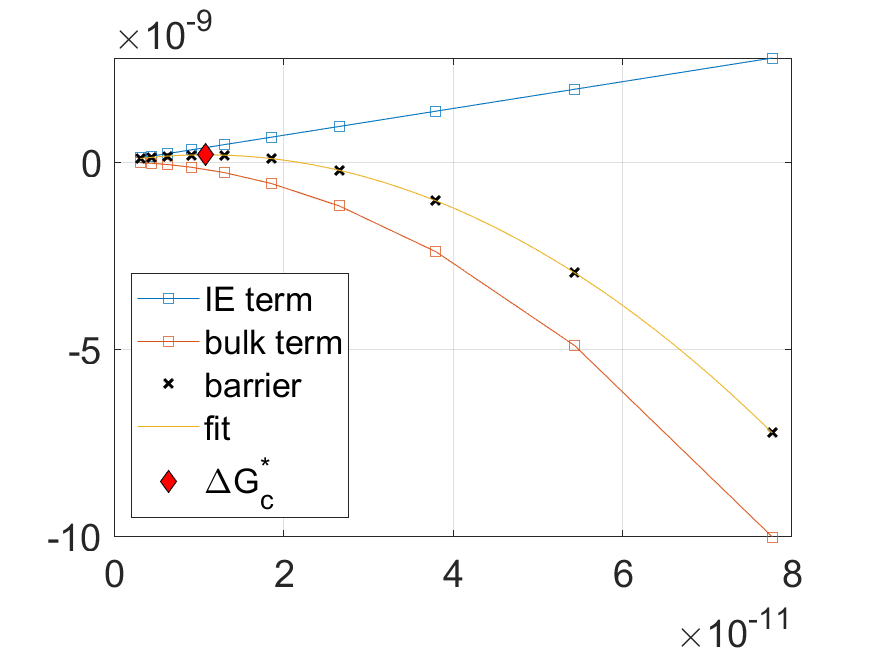
\includegraphics[width=0.4\textwidth]{NPA_calc_DGcrit.png}};
%		
%		\draw node[inner sep=0] at (-0.7,1) {(a)} ;
%		\draw node[left,inner sep=0] at (img.north west) {(b)} ;
%		\draw node[inner sep=0] at (img.west) {$\Delta G$} ;
%		\draw node[inner sep=0] at (img.south) {$\Delta x$} ;
%	\end{tikzpicture}
	
% NUCLEUS_ON_GB_ANNOTATED
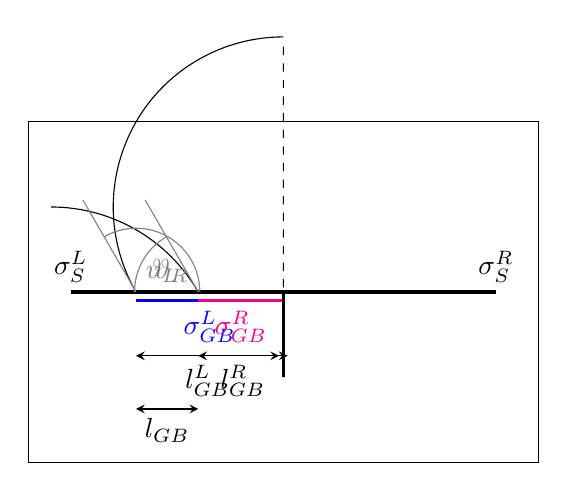
\begin{tikzpicture}[scale=2.7]
	\def\thl{120}
	\def\thr{-60}
	\def\R{0.8}
%	\tikzmath{ \RL = 0.4/sin(\thl) ; \RR = 0.7/sin(-\thr) ; }
	\tikzmath{ \cplX = -sin(\thl/2)*\R ; \cprX = sin(\thr/2)*\R ; }
	\path (-1,0) coordinate (al);
	\path (1,0) coordinate (ar);
	\path (0,0) coordinate (c);
	\path (0,-0.4) coordinate (cb);
	\path (\cplX,0) coordinate (cpl);
	\path (\cprX,0) coordinate (cpr);
	
	\draw[very thick, blue] ($(cpl)+(0,-0.04)$) -- node[midway,below] {$\sigma_{GB}^L$} ($(c)+(0,-0.04)$);
	\draw[very thick, magenta] ($(cpr)+(0,-0.04)$) -- node[midway,below] {$\sigma_{GB}^R$} ($(c)+(0,-0.04)$);		
	\draw[very thick] (al) -| (cb) |- (ar);
	\draw (cpl) arc (\thl+90:90:\R) node (toppoint) {};
	\draw[dashed] (toppoint) -- (c) ;
	\draw (cpr) arc (90+\thr:90:\R);
	\draw[gray] (cpl) node[above right] {$\vartheta_L$} -- ++(\thl:0.5);
	\draw[gray] (cpr) node[above left] {$\vartheta_R$}-- ++(180+\thr:0.5);
	\draw[gray] ($(cpl)+(0.3,0)$) arc (0:\thl:0.3);
	\draw[gray] ($(cpr)+(-0.3,0)$) arc (180:180+\thr:0.3);
	\draw node[above] at (al) {$\sigma_{S}^L$};
	\draw node[above] at (ar) {$\sigma_{S}^R$};
	\draw (-1.2,-0.8) rectangle (1.2,0.8);
	
	\def\vshift{-0.3}
	\draw[stealth-stealth] ($(cpr)+(0,\vshift)$) -- node[midway,below] {$l_{GB}^R$} ($(c)+(0.02,\vshift)$);	
	\draw[stealth-stealth] ($(cpl)+(0,\vshift)$) -- node[midway,below] {$l_{GB}^L$} ($(c)+(-0.02,\vshift)$);	
	\draw[stealth-stealth] ($(cpl)+(0,-0.55)$) -- node[midway,below] {$l_{GB}$} ($(cpr)+(0,-0.55)$);	
\end{tikzpicture}
	

%% CIRCLE_on_GB
%\begin{tikzpicture}
%	\begin{axis}[
%		axis equal,
%		axis line style={draw=none},
%		xtick=\empty,
%		ytick=\empty,
%		declare function={
%			yshift1=0.2;
%			yshift2=-0.6;
%			n=4;
%			nsoa=0;
%			rot1 = 30;
%			rot2 = rot1;
%			d=nsoa/(n^2-1);
%			aniso1(\t)=1+d*cos(n*(\t-rot1));
%			daniso1(\t)=-n*d*sin(n*(\t-rot1));
%			Wulffx1(\t) = aniso1(\t)*cos(\t) - daniso1(\t)*sin(\t);
%			Wulffy1(\t) = aniso1(\t)*sin(\t) + daniso1(\t)*cos(\t);
%			aniso2(\t)=1+d*cos(n*(\t-rot2));
%			daniso2(\t)=-n*d*sin(n*(\t-rot2));
%			Wulffx2(\t) = aniso2(\t)*cos(\t) - daniso2(\t)*sin(\t);
%			Wulffy2(\t) = aniso2(\t)*sin(\t) + daniso2(\t)*cos(\t);
%		},
%		]
%		\begin{scope}
%			\clip (axis cs: -2,5) rectangle (axis cs:0,0);
%			\addplot[domain=-pi:pi, samples=150, smooth, thick,red] ({Wulffx1(deg(x))},{Wulffy1(deg(x))+yshift1});
%		\end{scope}
%		
%		\begin{scope}
%			% \clip (axis cs: -2,-5) rectangle (axis cs:0,0);
%			\clip (axis cs: 0,0) -- (axis cs: 0,2) -- (axis cs: 2,2) -- (axis cs: 2,-2) -- (axis cs: -2,-2) -- (axis cs: -2,0) -- cycle (axis cs: 0,0) ;
%			\addplot[domain=-pi:pi, samples=150, smooth,red,dashed,thin] ({Wulffx1(deg(x))},{Wulffy1(deg(x))+yshift1});
%		\end{scope}
%		
%		\begin{scope}
%			\clip (axis cs: 0,5) rectangle (axis cs:2,0);
%			\addplot[domain=-pi:pi, samples=150, smooth,thick,blue] ({Wulffx2(deg(x))},{Wulffy2(deg(x))+yshift2});    
%		\end{scope}
%		
%		\begin{scope}
%			% \clip (axis cs: 0,-5) rectangle (axis cs:2,0);
%			\clip (axis cs: 0,0) -- (axis cs: 2,0) -- (axis cs: 2,-2) -- (axis cs: -2,-2) -- (axis cs: -2,2) -- (axis cs: 0,2) -- cycle (axis cs: 0,0) ;
%			\addplot[domain=-pi:pi, samples=150, smooth,blue,dashed, thin] ({Wulffx2(deg(x))},{Wulffy2(deg(x))+yshift2});    
%		\end{scope}
%		
%		\path coordinate (C1) at (axis cs:0,yshift1);
%		\path coordinate (C2) at (axis cs:0,yshift2);
%		\path coordinate (B1) at (axis cs:-2,0);
%		\path coordinate (B2) at (axis cs:2,0);
%		\path coordinate (B3) at  (axis cs:0,-2);
%		\path coordinate (zz) at  (axis cs:0,0);
%		% \draw[red] (B1) -- (zz);
%		% \draw[blue] (B2) -- (zz);
%		\draw[<->,thick,red] (axis cs:-0.2,0) -- (axis cs:-0.2,yshift1);
%		\draw[<->,thick,blue] (axis cs:0.2,0) -- (axis cs:0.2,yshift2);
%		
%		\draw[fill,red] (C1) circle (3pt);
%		\draw[fill,blue] (C2) circle (3pt);
%		
%		\draw (axis cs:-1.5,0.5) node [circle,draw,minimum size=6] {$\mathit{1}$};
%		\draw (axis cs:-0.5,0.6) node [circle,draw,minimum size=6] {$\mathit{2}$};
%		\draw (axis cs:-1.5,-0.5) node [circle,draw,minimum size=6]  {$\mathit{3}$};
%		\draw (axis cs:1.5,-0.5) node [circle,draw,minimum size=6] {$\mathit{4}$};
%		
%		\draw[thick] (B1) -- (B2);
%		\draw[thick] (zz) -- (B3);
%		\draw[dashed] (zz) -- (axis cs:0,2);
%
%	\end{axis}
%\end{tikzpicture}
	
\end{document}
